\begin{frame}{AGRET}{Agent-Group-Role-Environment-Time}
\begin{itemize}
    \item \textbf{Objective}: evolve the ABM so as to naturally take into account the temporal dimension as well as the spatial and organizational dimensions
    \item \textbf{Hypothesis}: 
    \begin{itemize}
        \item time representation
        \item medium for the exchange of temporal information between agents
        \item a visibility on the temporal dimension
    \end{itemize}
    \item \textbf{Constraints}:
    \begin{itemize}
        \item equal consideration of the 3 dimensions: spatial, temporal, social, etc.
        \item integrate within the existing multi-agent system
    \end{itemize}
    \item \textbf{Proposal}:
    \begin{itemize}
        \item an interaction environment for storing and accessing information
        \item an interaction model that allows the link between the agents and the interaction environment
        \item an approach that articulates the spatial, organizational and temporal dimensions
    \end{itemize}
\end{itemize}

\note{
Notre ojectif est de faire évoluer le paradigme SMA de manière à prendre en compte naturellement la dimension temporelle au même titre que les dimensions spatiale et organisationnelle. Notre première contribution concerne la représentation du temps. Elle consiste en la proposition d’un support permettant l’échange d’informations entre les agents. L’échange d’informations spatiales et sociales est déjà existante et couramment utilisé dans les SMA. Cependant, l’échange d’informations sur la dimension temporelle reste une axe de recherche à explorer. Ce support devrait permettre aux agents d’avoir, en plus de la visibilité sur le spatial et sur le social qui existe déjà,  une visibilité sur la dimension temporelle. Pour cela, le support devrait prendre en compte les contraintes suivantes : les 3 dimensions devraient être pris en compte au même titre. De plus, le support d’interaction temporel doit être intégrable facilement au sein du système multi-agent déjà existant, sans réécriture de tout le code du modèle de simulation ou du simulateur. Il devra compléter le rôle de l’ordonnanceur de la simulation qui gère déjà le temps au niveau de la simulation.
\par Pour mettre en place ce nouveau support au sein du système existant, nous proposons un ensemble de solutions qui s’articule sur trois points:
\begin{itemize}
    \item un milieu d’interaction qui sert au stockage et à l’accès aux informations
    \item un modèle d’interaction qui permet le lien entre les agents et le milieu d’interaction
    \item une approche permettant d’articuler les 3 dimensions spatiale, organisationnelle et temporelle.
\end{itemize}
}
\end{frame}

\begin{frame}{AGRET}{An interaction medium}
\begin{itemize}
    \item Modeling time as an environment
    \item How does this temporal environment position itself regarding to the scheduler of the simulation?
    \begin{itemize}
        \item the temporal environment is interfaced between the agent and the scheduler of the simulation
        \item the temporal environment breaks the direct link between the agent and the scheduler
        \item The temporal environment does not replace the scheduler:
        \begin{itemize}
            \item The temporal environment and the scheduler are complementary
            \item The temporal environment is located at the simulation model level while the scheduler is located at the simulation platform level
        \end{itemize}
        \item The temporal environment manages the representation of time and the exchange of temporal information while the simulation scheduler manages the activation cycle of the simulation
    \end{itemize}
\end{itemize}

\note{
En partant du constat que les dimensions spatiale et organisationnelle sont modélisé, la plupart du temps, sous forme d’environnements, nous proposons une modélisation du temps sous forme d’environnement. Nous appelons cet environnement : l’environnement temporel. Mais comment se positionne cet environnement temporel par rapport à l’ordonnanceur de la simulation qui relève également de la dimension temporelle?
Comme je l’ai expliqué dans le diaporama d’avant, le mécanisme d'activation des agents se fait par lien direct entre l'agent et le sous-système que l'on appelle l'ordonnanceur. Désormais, dans notre proposition, l'environnement temporel vient s'interfacer entre l'agent et l'ordonnanceur de la simulation. Cette nouvelle approche casse le lien direct qui existe entre ces derniers. L'approche que nous proposons ne remplace pas l'ordonnanceur de la simulation qui gère les mécaniques d'avancement du temps simulé et l'activation des agents et de la simulation. Au contraire, elle vient compléter le fonctionnement de ce dernier. \textbf{L'environnement temporel gère la représentation du temps et les échanges d'informations temporelles tandis que l'ordonnanceur de la simulation gère le cycle d'activation de la simulation}. Nous distinguons donc bien ce qui relève du modèle de simulation de ce qui relève de la plateforme de simulation. L’environnement temporel se situe au niveau du modèle de simulation tandis que l’ordonnanceur se situe au niveau du simulateur.
}
\end{frame}

\begin{frame}{AGRET}{An interaction model}
\begin{itemize}
    \item For the link between the agent and the temporal environment
    \item Influence/Reaction model
    \begin{itemize}
        \item perception, deliberation, influence
        \item Influence:
        \begin{itemize}
            \item do not directly alter the environment
            \item represent an agent's desire to see the environment changed in some way, a way of trying to make a difference
        \end{itemize}
        \item clear distinction between agents and environment
    \end{itemize}
\end{itemize}

\note{Le modèle d'intéraction permet de faire le lien entre l'agent et l'environnement temporel. Nous proposons un modèle d’interaction de type influence/réaction. Ce modèle diffère de l’approche classique action/réaction qui est fréquement utiliser pour modéliser l’interaction entre l’agent et son environnement. En effet, si le cycle comportemental classique d’un agent se résume en trois phases: perception, délibération, action aboutit à une transformation directe de l’environnement. Dans le modèle influence réaction, il aboutit à une influence. Cet influence diffère de l’action dans le sens où elles ne modifient pas directement l'environnement. Elles représentent le souhait d'un agent de le voir modifié d'une certaine façon, un moyen d'essayer de changer le cours des choses.  Ce modèle distingue alors bien tout ce qui relève de l’agent de tout ce qui relève de l’environnement. En d'autres termes, un agent ne peut que décider de l'action suivante à faire. C'est à son environnement de déterminer les conséquences de cette dernière. L'environnement dispose alors de ses propres modalités de fonctionnement qui s'imposent à l'agent. Par exemple : un agent décide de faire déplacer un objet de l’environnement, mais c'est son environnement (son corps et son environnement extérieur) qui exécute le déplacement.
Nous y reviendrons plus en détails après.
}
    
\end{frame}

\begin{frame}{AGRET}{An approach allowing to articulate the 3 dimensions}
\begin{itemize}
    \item AGR (Agent-Group-Role): one of the most well-known organizational approaches in ABM
    \begin{itemize}
        \item 3 notions :
            \begin{itemize}
                \item Agent : an active and communicating entity, plays a role in one or more groups, can take on several roles and can be a member of several groups
                \item Group :  set of agents sharing common characteristics
                \item Role : abstract representation of a functional position of an agent in a group
            \end{itemize}
        \item \textbf{Advantages}: generic and minimalist
        \item \textbf{Limit}: Do not take the environment into account
    \end{itemize}
    \item AGRE (Agent-Group-Role-Environment):  
    \begin{itemize}
        \item  complements the corporal/physical situated aspect to the social situated aspect of AGR
        \item take into account two of the three dimensions: the spatial dimension and the organizational dimension.
    \end{itemize}
\end{itemize}

\note{
Une approche permettant d’articuler les 3 dimensions spatiale, organisationnelle et temporelle: une des approches organisationnelles les plus connues dans le domaine des SMA est l’approche AGR (Agent-Groupe-role). Son organisation s'articule autour de trois notions \begin{itemize}
    \item Agent : Un agent est une entité active et communiquante. Il joue un \emph{rôle} dans un ou plusieurs groupes, peut tenir plusieurs rôles et peut être membre de plusieurs groupes.
    \item Groupe : Un groupe est un ensemble d'agents partageant des caractéristiques communes. Un groupe est utilisé comme un contexte pour un modèle d'activités ou pour partitionner des organisations. Deux agents peuvent communiquer si et seulement s'ils appartiennent au même groupe. Un agent peut appartenir à plusieurs groupes. Cette fonctionnalité permet de définir des structures organisationnelles.
    \item Rôle : Le rôle est la représentation abstraite d'une position fonctionnelle d'un agent dans un groupe. Un agent doit jouer un rôle dans un groupe et peut en jouer plusieurs dans ce même groupe. Les rôles sont locaux aux groupes et un rôle doit être demandé par un agent. Un même rôle peut être joué par plusieurs agents.
\end{itemize}
AGR est une des approches organisationnelles comportementalistes les plus connues des SMA. Elle a l'avantage d'être minimaliste et générique. Cependant, elle a été critiquée par ces mêmes auteurs du fait qu'elle ne prenne pas en compte le concept d'environnement. Pourtant, il s'agit d'un concept important dans le cadre des interactions dans les SMA et plus particulièrement dans le contexte d'agents situés. 

\par AGRE vient compléter l’aspect situé corporel à l’aspect situé social d'AGR. Dans AGRE, un agent possède un ensemble de modes qui peuvent être sociaux ou physiques. Les modes sociaux, sont considérés comme des interfaces sociaux permettant d'agir en groupe et sont appelés rôles. De la même manière, les modes physiques sont considérés comme des interfaces physiques permettant d'agir dans une zone. D'une manière plus générale, les modes sont des interfaces permettant d'agir dans les espaces.
Ainsi, AGRE permet de prendre en compte deux des trois dimensions : la dimension spatiale et la dimension organisationnelle.
Dans cette thèse, nous proposons d’étendre AGRE de manière à y intégrer la prise en compte de la dimension temporelle : nous nommons notre approche AGRET : Agent Groupe Rôle Environnement Temps. 

}
    
\end{frame}

\begin{frame}{AGRET}{Agent-Group-Role-Environment-Time}
We take the basic principles of AGRE and add the time dimension

\begin{figure}
	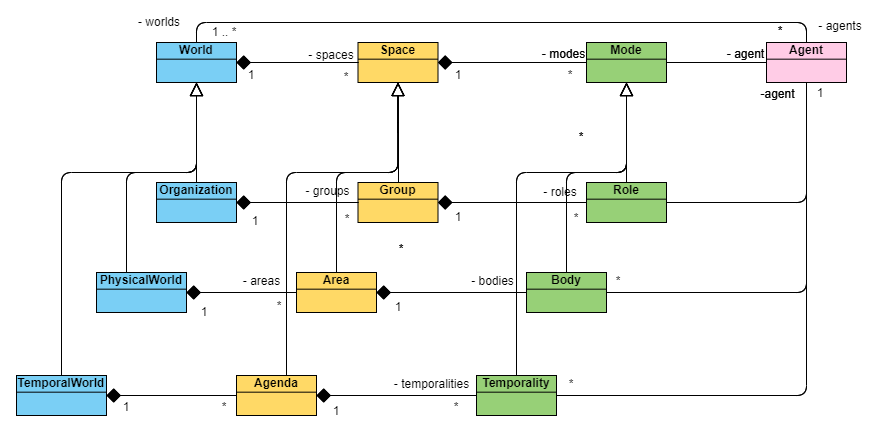
\includegraphics[width=\textwidth]{figures/agret.png}
\end{figure}

\note{Dans leur article  Ferber et al. considèrent uniquement deux types de monde : les organisations (environnements sociaux) qui sont composées d'un ensemble de groupes, et le monde physique (environnements physiques) qui se compose de zones. Néanmoins, ils évoquent la possibilité d'existence d'autres types de monde et d'autres types d'espace qu'ils ne décrivent pas dans leur article \cite{FerberMB04}. Dans \gls{agret}, nous reprenons les principes de base d'\gls{agre} et nous rajoutons la dimension temps. Nous définissons alors un nouveau type d'espace qui est de type temporel et que nous appelons \emph{agenda}. Comme dans \gls{agr} et \gls{agre}, les agents sont situés dans les espaces et peuvent y agir à travers les modes. Si un mode dans une zone est appelé corps (body), un mode dans un groupe est appelé rôle (role), nous appelons un mode dans un agenda une \textbf{temporalité (temporality)}. Un nouveau type de monde vient également s'ajouter à ces deux types de monde déjà existants dans \gls{agre}: le monde temporel (temporal world).
La figure montre un diagramme UML simplifié qui représente les relations entre mondes, espaces, zones, groupes, agendas, modes, corps, rôles et temporalités.
\par Après avoir proposé une approche permettant d’articuler les 3 dimensions spatiale, organisationnelle et temporelle, nous allons zoomer un peu plus sur le milieu d’interaction, c’est-à-dire l’environnement temporel pour voir comment gérons les mécaniques internes à l’environnement temporel.
}    
\end{frame}


\begin{frame}{Interaction environment}{The temporality model for structuring the temporal environment}
Ajouter schéma modèle à temporalité vs structuration de l'environnement temporel


\note{
Afin de structurer notre environnement temporel, nous nous reposons sur une approche qui à l’origine est  destiné uniquement à l’ordonnancement de la simulation : le modèle à temporalité. Le modèle à temporalité est un type particulier d'approche d'ordonnancement du temps dans les simulations multi-agent. C'est une approche dite expressive, car elle permet à l'agent de décrire lui-même sa propre dynamique temporelle. C’est-à-dire qu’elle permet à l’agent d’indiquer à l’ordonnanceur de la simulation à quelle moment il souhaite être réveillé. Cela se fait par définition d'une structure de donnée appelée \emph{temporalité}. Un agent définit une ou plusieurs temporalités en fonction de la complexité et de la diversité des activités qu'il souhaite entreprendre. Son comportement résulte de l'exécution de l'ensemble de ces activités. Au niveau de l'ordonnanceur, une temporalité est la description d'une série d'occurrences temporelles. Cette description spécifie les points de l'axe du temps, pour lesquels l'agent souhaite que l'ordonnanceur de la simulation déclenche l'exécution de son comportement. Le traitement interne des temporalités par l'ordonnanceur fait intervenir deux structures de donnée comme le montre la figure. 
\begin{itemize}
    \item Slot temporel : Élément d’ancrage correspondant à un point de l’axe du temps sur lequel  le  simulateur  va  être  amené  à  déclencher  l’exécution  du  code  de comportement d’un agent.
    \item Tempo : Structure  regroupant  l’ensemble  des  temporalités  qui  à un instant donné sont situées sur  un même slot  temporel et  qui ont la même valeur de période. C’est cette valeur de période qui caractérise le tempo en traduisant le fait que les temporalités qu’il comporte ont toutes le même \say{rythme}.
\end{itemize}
L’ordonnanceur fait progresser  le temps simulé  en l’emmenant successivement sur chacune des positions signalées par un slot temporel. À chaque slot temporel, tous les tempos sont traités. Cela produit l’exécution de tous les  comportements associés  aux  temporalités qu’ils comportent.
 Nous reprenons ces mêmes principes de base dans notre modèle d'environnement temporel (temporalité, slot, tempo). Ils nous servent à structurer les informations temporelles contenues dans ce milieu d'interaction. Ils permettent également la mise en place de la mécanique environnementale. 
 \par Dans l'environnement temporel, la notion de temporalité est un peu plus étendue. Nous la définissons comme étant la \textbf{représentation de l'agent dans l'environnement temporel}, au même titre que le corps de l'agent dans l'environnement spatial ou le rôle dans l'environnement social.
\par Le corps possède une localisation spatiale dans l'environnement physique. Son déplacement se traduit par la modification de sa localisation spatiale. De la même manière, une temporalité possède une localisation temporelle dans l'environnement temporel. Son déplacement se traduit par la modification de sa localisation temporelle. C'est cette notion de localisation temporelle dans l'environnement temporel qui est équivalente à la notion de temporalité dans le modèle à temporalité (au niveau de l'ordonnanceur). Cette localisation temporelle est définie par $t=\{id,d,f,p,v\}$ où $id,d,f,p,v$ sont les paramètres obligatoires de la temporalité qui permettent d'établir l'axe temporel des agents du système. Son déplacement dans l'environnement temporel se traduit alors par la modification de sa localisation temporelle, plus précisément par la modification des différents paramètres $id,d,f,p,v$. Nous y revenons plus en détail dans la sous-section \ref{subsec:Application à l'environnement temporel}. $d,f,p,v$ sont des paramètres objectifs. C'est-à-dire que leur valeur se calcule à partir de données réelles, sans prendre en compte du ressenti ou des préjugés de l'agent. D'autres paramètres optionnels peuvent être rajoutés en fonction des besoins et du but du modélisateur. Ces paramètres peuvent être objectifs ou subjectifs. Par exemple : le coût, la criticité, la priorité ou la pondération sont des paramètres subjectifs. Elles correspondent à l'évaluation de l'importance que l'agent accorde à l'occurrence temporelle, à un ressenti de l'agent. Un exemple de paramètre optionnel objectif est la longueur prévisionnelle de la file d'attente. Nous verrons un exemple d'utilisation de ces paramètres optionnels dans notre deuxième contribution que nous présentons dans le chapitre \ref{chap: Anticipation} suivant.
}
    
\end{frame}

\begin{frame}{Interaction environment}{The temporality model for structuring the temporal environment}

\note{
\par Dans l'approche originale du modèle à temporalité proposé par Payet et al., aucun support n'a été prévu pour le stockage des informations passées. L'ordonnanceur calcule les prochaines dates de déclenchement des temporalités futures avant chaque avancement du temps. Il supprime également les temporalités passées, car elles n'interviennent plus dans le cycle d'activation de la simulation. De plus, il n'existe pas de mécanisme permettant la perception d'informations sur la dynamique d'activation temporelle des agents. En effet, ces fonctionnalités ne sont pas nécessaires compte tenu de l'objectif pour lequel l'approche a été originellement conçue : l'ordonnancement de la simulation. 
\par Cependant, le stockage et la perception des informations temporelles sont indispensables dans l'usage que nous en faisons.  Nous travaillons alors sur la refonte de l'ancien modèle, en l'élargissant avec deux aspects. Nous mettons en place un support permettant aux agents, non seulement de partager des informations sur leur dynamique temporelle (comme c'est déjà le cas dans le modèle à temporalité), mais également de stocker et de percevoir des informations positionnées sur le passé, sur le présent et sur le futur. 
\par Au niveau de l'ordonnanceur, dans le modèle à temporalité, les créations et les modifications de temporalités sont immédiatement traitées par l’ordonnanceur. Pour cela, il actualise les structures de représentation lui servant à déterminer la façon dont le temps simulé va s’écouler et les activations à réaliser au cours de sa progression. Ainsi, comme dans la plupart des approches classiques d'ordonnancement du temps dans les simulations agents, l'activation des agents par l'ordonnanceur se fait par lien direct entre ce dernier et l'agent à activer. Dans l'approche que nous proposons, nous cassons ce lien direct en interfaçant l'environnement temporel entre l'agent et l'ordonnanceur. Le processus de modification ou de création de temporalité se fait alors comme la suivante : à un slot de temps $s$ : 
\begin{enumerate}
    \item L'ordonnanceur traite les demandes d'activation d'agents pour le slot courant $s$. Il réveille les agents qui se sont exprimés vouloir s'activer à $s$.
    \item Les agents réveillés enclenchent leur cycle perception-décision-action/influence. Ils perçoivent leur contexte d'activation (phase de perception). Notamment au niveau de l'environnement temporel, ils perçoivent les informations relatives à l'action qu'ils ont prévu d'effectuer à ce slot $s$. Ils sont libres de choisir par eux même d'agir ou non (phase de décision). Ils définissent, modifient ou suppriment une ou plusieurs localisations temporelles au niveau de l'environnement temporel (phase d'influence). Ces définitions ou ces modifications de localisations temporelles ne sont pas traitées immédiatement par l'environnement temporel. 
    \item  L'environnement temporel attend la fin de l'activation de tous les agents du système pour traiter l'ensemble des définitions et des modifications de localisations temporelles. Il s'occupe de leur stockage et de l'actualisation des structures de représentation de la dynamique temporelle des agents (rattachement à un slot, regroupement en tempos, etc. ). Nous y revenons plus en détail dans \ref{sec:Intégration du modèle influence-réaction pour la simulation}.
    \item  L'ordonnanceur est  mis à jour en fonction des données contenues dans l'environnement temporel. Il actualise les structures de représentation lui servant à déterminer la façon dont le temps simulé va s’écouler et les activations à réaliser au cours de sa progression.
\end{enumerate}
\textbf{Tout ce processus se fait sur le même slot de temps}.

Dans l'approche que nous proposons, la localisation temporelle est traitée et stockée au niveau de l'environnement temporel afin que les agents puissent non seulement les créer ou les modifier, mais également les percevoir. En complément à cela, nous laissons à l'ordonnanceur de la simulation le soin de s'occuper de la gestion de l'écoulement du temps et de l'activation des agents. 
}
\end{frame}

\begin{frame}{Interaction model}{The influence/Reaction Model}

\note{
citeauthor{FerberST09} \cite{FerberST09} critiquent \gls{agre} et toutes les familles de modèles de type \gls{agr} (dont \gls{agret}) du fait qu'ils ne fournissent pas de théorie de l'action qui prendrait en compte les actions concurrentes. Afin d'y remédier, une des solutions proposées consiste en l'utilisation du modèle influence/réaction \cite{ferber1996influences} \cite{FerberST09} pour gérer l’interaction entre l’agent et l’environnement. Dans l'approche que nous proposons, nous faisons une claire distinction entredeux phases : phase d'influence et phase de réaction. Plus particulièrement, 
\citeauthor{FerberMB04} proposent une \say{simplification} et une clarification du modèle influence/réaction dans le cadre de la simulation multi-agent. Le modèle s'appelle \gls{irm4s}. Il s'agit d'une approche adaptée dans un contexte de simulation multi-agent.
\par Comme dans toute approche de type influence/réaction, dans \gls{irm4s}, le cycle comportemental de l'agent aboutit à la production d'influences. Cependant, dans le modèle influence/réaction, les agents perçoivent ce qui les influence, mais ne sont pas influencés par l'état de l'environnement. Contrairement à cela, \gls{irm4s} prend en compte la perception locale et subjective de son environnement par un agent. Cela se traduit par la présence de l'état de l'ensemble des variables environnementales $\Sigma$, en entrée à la fonction $Behaviour_a$
\medbreak
\par Au niveau agent, les trois (3) fonctions composant la fonction behaviour deviennent alors :
\begin{itemize}
    \item $Percept_a : \Sigma \times \Gamma \mapsto P_a$. Dans le modèle classique d'influence/réaction, cette fonction prend en entrée uniquement des influences. Contrairement à cela, dans \gls{irm4s}, cette fonction prend en entrée, en plus des influences, l'ensemble des variables environnementales, c'est-à-dire l'état de l'environnement. 
    \item Les fonctions de mémorisation et de décision quant à elles restent inchangées.
\end{itemize}
Cette perception de l'état de l'environnement est importante dans l'approche que nous proposons. Elle permet aux agents d'extraire un ensemble d'informations spatiales, sociales et temporelles à partir des supports d'interaction qui dans notre cas sont les environnements. Ces informations servent par la suite dans le cadre du raisonnement anticipatif. Ce raisonnement est notre deuxième proposition que nous décrivons dans le chapitre \ref{chap: Anticipation} suivant.
\par Ce modèle a été particulièrement conçu pour répondre au problème de la simultanéité. Il a également l'avantage de faire le lien entre les dynamiques des niveaux micro (agent) et macro (système multi-agent). De plus, il sépare, de manière claire tout ce qui relève de l'agent de tout ce qui relève de l'environnement.
\par Pour rappel, son principe se base sur l'idée selon laquelle un agent ne peut pas directement changer l'état du monde, mais peut tout simplement influencer ses dynamiques. En d'autres termes, un agent ne peut que décider de l'action suivante à faire. C'est à son environnement de déterminer les conséquences de cette dernière. L'environnement dispose alors de ses propres modalités de fonctionnement qui s'imposent à l'agent.
Par exemple, un agent veut envoyer un message et effectue l'opération qui consiste à l'envoyer. Son environnement se charge de le transmettre et de le délivrer à son destinataire. De la même manière, un agent décide de bouger, mais c'est son environnement (son corps et son environnement extérieur) qui exécute le déplacement. En suivant la même logique au niveau de l'environnement temporel du modèle \gls{agret} : un agent peut définir une localisation temporelle. Cependant,  c'est son environnement temporel qui se charge de la créer ou pas, en fonction des autres influences produites par les autres agents, en fonction des lois de l'environnement temporel, etc. Ainsi, l'environnement réagit aux influences produites par les agents. 
\par Cette séparation stricte de tout ce qui relève de l'agent et tout ce qui relève de l'environnement se traduit par la séparation du cycle d'activité classique d'un simulateur utilisant un type d'ordonnancement à temps discret en deux phases : 
\begin{itemize}
   \item Une phase d’activation de l’environnement durant laquelle le simulateur doit mettre à jour l’horloge virtuelle, initialiser le prochain cycle, etc.;
    \item Une phase d'activation des agents durant laquelle l'agent applique le processus itératif : perception, mémorisation, décision. 
\end{itemize}
}
    
\end{frame}

\begin{frame}{Interaction model}{Time constrained and non-constrained environment}

\note{
\par Dans la plupart des simulateurs, la phase d'activation de l'environnement se déroule en début du cycle d'activité de la simulation. Cela est dû au fait que la plupart des environnements a besoin de calculer son nouvel état en début d'un cycle (instant $t$), avant l'activation des agents. Ces calculs doivent  s'établir sur l'intervalle de temps qui s'est écoulé depuis la dernière activation, c'est-à-dire dans l'intervalle $]t-dt, t]$. Ces environnements ont des états qui évoluent dans le temps en fonction des lois inertielles qui leur sont propres, et des influences qu'exercent les agents. Ce sont donc, en quelque sorte, des \textbf{environnements contraints par le temps}.
\par Dans notre contexte, la mise en place d'un nouveau type d'environnement qui est l'environnement temporel vient chambouler le fonctionnement de ce cycle classique d'ordonnancement de la simulation. Par définition, l'état de l'environnement temporel détermine la dynamique d'écoulement du temps. Par conséquent, son état évolue hors du temps. En effet, l'état dynamique de l'environnement temporel reste soumis à des lois inertielles (la mécanique des slots temporels) et aux influences exercées par les agents sous forme de \say{localisations temporelles}. Cependant, cela se fait indépendamment de l'intervalle de temps écoulé depuis les derniers calculs. Seule la connaissance du dernier slot temporel courant est nécessaire pour servir de point de référence aux nouvelles localisations temporelles exprimées par les agents, et aux déplacements des slots temporels périodiques. Ainsi, \textbf{l'environnement temporel n'est pas un environnement contraint par le temps}. De manière concrète, le calcul du prochain slot d'activation temporel ($t+dt$) est fonction de l'ensemble des influences exercées par les agents durant le slot temporel courant ($t$) ainsi que des lois de l'environnement temporel. Le traitement des calculs au niveau de l'environnement temporel doit alors se faire obligatoirement avant, $t+dt$ car il permet de déterminer $t+dt$. Plus précisément, ce traitement doit se faire à la fin du cycle courant, car il faut attendre la fin du cycle d'activation de tous les agents et le calcul des réactions de l'environnement.
\par Ce raisonnement nous amène donc aux conclusions suivantes : 
\begin{itemize}
    \item les environnements contraints par le temps doivent être activés en début de cycle pour leur permettre de calculer leur nouvel état sur l'intervalle de temps écoulé $]t-dt ; t]$.
    \item les environnements non contraints par le temps doivent être activés en fin de cycle pour leur permettre de calculer leur nouvel état en fonction du dernier slot temporel courant $t$.
\end{itemize}
\par Ainsi, aux deux phases du cycle d'activation classique de la simulation s'ajoute alors une troisième phase comme le montre la figure \ref{Fig: Cycle_activité}. Les trois nouvelles phases du cycle d'activation de la simulation sont :
\begin{enumerate}
    \item la phase d'activation des environnements contraints par le temps sur l'intervalle de temps $]t-dt ; t]$; 
    \item la phase d'activation des agents sur le slot temporel courant $t$;
    \item la phase d'activation des environnements non contraints par le temps sur la considération que $t$ vient d'être passé.
\end{enumerate}
}
    
\end{frame}

\begin{frame}{Frame Title}
    
\end{frame}